
\chapter{Introduction and main results\label{chap:Introduction-and-overview}}

\addcontentsline{lof}{chapter}{Introduction and overview\lofpost}
%\addcontentsline{lot}{chapter}{Introduction and overview\lofpost}

\singlespacing 
\epigraph{
If all this damned quantum jumping were really to stay,  I should be sorry I ever got involved with quantum theory.}
{Erwin Schr\"odinger\\ \textit{Brit. J. Philos. Sci. III}, 109 (1952)} 
\doublespacing  \noindent Bohr conceived of quantum jumps \citet{Bohr1913} in 1913, and while
Einstein elevated their hypothesis to the level of a quantitative
rule with his AB coefficient theory \citep{Einstein1916,Einstein1917},
Schrödinger strongly objected to their existence \citep{Schrodinger1952}.
The nature and existence of quantum jumps remained a subject of controversy
for seven decades until they were directly observed in a single system
\citep{Nagourney1986,Sauter1986,Bergquist1986}. Since then, quantum
jumps have been observed in a variety of atomic \citep{Basche1995,Peil1999,Gleyzes2007,Guerlin2007}
and solid-state \citep{Jelezko2002,Neumann2010,Robledo2011,Vijay2011,Hatridge2013}
systems. Recently, quantum jumps have been recognized as an essential
phenomenon in quantum feedback control \citep{Deleglise2008,Sayrin2001},
and in particular, for detecting and correcting decoherence-induced
errors in quantum information systems \citep{Sun2013,Ofek2016}.

Here, we focus on the canonical case of quantum jumps between two
levels indirectly monitored by a third --- the case that corresponds
to the original observation of quantum jumps in atomic physics \citep{Nagourney1986,Sauter1986,Bergquist1986},
see the level diagram of Fig.~\ref{fig:setup}a. A surprising prediction
emerges according to quantum trajectory theory (see \citet{Carmichael1993,Porrati1987,Ruskov2007}
and Chapter\,\ref{chap:Quantum-Trajectory-Theory}): not only does
the state of the system evolve continuously during the jump between
the ground $\ket{\mathrm{G}}$ and excited $\ket{\mathrm{D}}$ state,
but it is predicted that there is always a latency period prior to
the jump, during which it is possible to acquire a signal that warns
of the imminent occurrence of the jump (see Chapter~\ref{chap:theoretical-description-jumps}
for the theoretical analysis and mathematical treatment). This advance
warning signal consists of a rare, particular lull in the excitation
of the ancilla state $\ket{\mathrm{B}}$. The acquisition of this
signal requires the time-resolved detection of\textit{ every} de-excitation
of $\ket{\mathrm{B}}$. Instead, exploiting the specific advantages
of superconducting artificial atoms and their quantum-limited readout
chain, we designed an experiment that implements with maximum fidelity
and minimum latency the detection of the advance warning signal occurring
before the quantum jump (see rest of Fig.~\ref{fig:setup}).

\section{Principle of the experiment \label{sec:Principle-of-the}}

First, we developed a superconducting artificial atom with the necessary
V-shape level structure (see Fig.~\ref{fig:setup}a and Section~\ref{sec:circuit-design}).
It consists, besides the ground level $\ket{\mathrm{G}}$, of one
protected, dark level $\ket{\mathrm{D}}$ --- engineered to not couple
to any dissipative environment or any measurement apparatus --- and
one ancilla level $\ket{\mathrm{B}}$, whose occupation is monitored
at rate $\Gamma$. Quantum jumps between $\left|\mathrm{G}\right>$
and $\left|\mathrm{D}\right>$ are induced by a weak Rabi drive $\Omega_{\mathrm{DG}}$
--- although this drive might eventually be turned off during the
jump, as explained later. Since a direct measurement of the dark level
is not possible, the jumps are monitored using the Dehmelt shelving
scheme \citep{Nagourney1986}. Thus, the occupation of $\left|\mathrm{G}\right>$
is linked to that of $\left|\mathrm{B}\right>$ by the strong Rabi
drive $\Omega_{\mathrm{BG}}$ ($\Omega_{\mathrm{DG}}\ll\Omega_{\mathrm{BG}}\ll\Gamma$).
In the atomic physics shelving scheme \citep{Nagourney1986,Sauter1986,Bergquist1986},
an excitation to $\ket{\mathrm{B}}$ is recorded with a photodetector
by detecting the emitted photons from $\ket{\mathrm{B}}$ as it cycles
back to $\G$. From the detection events --- referred to in the following
as ``clicks'' --- one infers the occupation of $\ket{\mathrm{G}}$.
On the other hand, from a prolonged absence of clicks (to be defined
precisely in Chapter~\ref{chap:theoretical-description-jumps}),
one infers that a quantum jump from $\ket{\mathrm{G}}$ to $\ket{\mathrm{D}}$
has occurred. Due to the poor collection efficiency and dead-time
of photon counters in atomic physics \citep{Volz2011}, it is exceedingly
difficult to detect every individual click required to faithfully
register the origin in time of  the advance warning signal. However,
superconducting systems present the advantage of high collection efficiencies
\citep{Vijay2012,Riste2013,Murch2013,Weber2014,Roch2014,deLange2014,Campagne2016-Fluorescence},
as their microwave photons are emitted into one-dimensional waveguides
and are detected with the same detection efficiencies as optical photons.
Furthermore, rather than monitoring the direct fluorescence of the
$\ket{\mathrm{B}}$ state, we monitor its occupation by dispersively
coupling it to an ancilla readout cavity. This further improves the
fidelity of the detection of the de-excitation from $\ket{\mathrm{B}}$
(effective collection efficiency of photons emitted from $\ket{\mathrm{B}}$).

\begin{figure}
\centering{}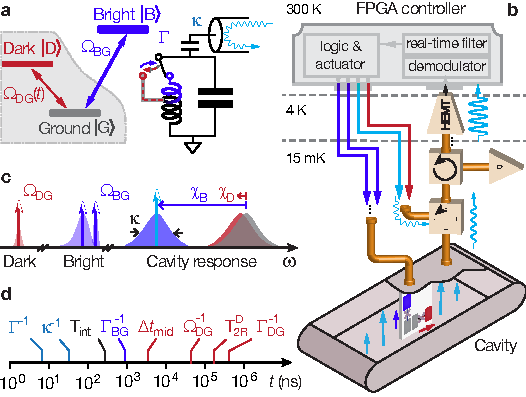
\includegraphics[width=130mm]{intro/1_setup} \caption[Principle of the experiment]{\label{fig:setup}\textbf{Principle of the experiment.} \textbf{a,}
Three-level atom possessing a hidden transition (shaded region) between
its ground $\ket{\mathrm{G}}$ and dark $\ket{\mathrm{D}}$ state,
driven by Rabi drive $\Omega_{\mathrm{DG}}(t)$. Quantum jumps between
$\ket{\mathrm{G}}$ and $\ket{\mathrm{D}}$ are indirectly monitored
by a stronger Rabi drive $\Omega_{\mathrm{BG}}$ between $\ket{\mathrm{G}}$
and the bright state $\ket{\mathrm{B}}$, whose occupancy is continuously
monitored at rate $\Gamma$ by an auxiliary oscillator (LC circuit
on right), itself measured in reflection by continuous-wave microwave
light (depicted in light blue). When the atom is in $\ket{\mathrm{B}}$,
the LC circuit resonance frequency shifts to a lower frequency than
when the atom is in $\ket{\mathrm{G}}$ or $\ket{\mathrm{D}}$ (effect
schematically represented by switch). Therefore, the probe tone performs
a $\ket{\mathrm{B}}$/not-$\ket{\mathrm{B}}$ measurement on the atom,
and is blind to any superposition of $\ket{\mathrm{G}}$ and $\ket{\mathrm{D}}$.
\textbf{b,} The actual atom and LC oscillator used in the experiment
is a superconducting circuit consisting of two strongly-hybridized
transmon qubits placed inside a readout resonator cavity at 15\,mK.
Control signals for the atom and cavity are supplied by a room-temperature
field-programmable gate array (FPGA) controller. This fast electronics
monitors the reflected signal from the cavity, and after demodulation
and filtering, actuates the control signals. The amplifier chain includes
circulators (curved arrows) and amplifiers (triangles and trapezoids).
\textbf{c,} Frequency landscape of atom and cavity responses, overlaid
with the control tones shown as vertical arrows. The cavity pull $\chi$
of the atom is nearly identical for $\ket{\mathrm{G}}$ and $\ket{\mathrm{D}}$,
but markedly distinct for $\ket{\mathrm{B}}$. The BG drive is bi-chromatic
in order to address the bright transition independently of the cavity
state. \textbf{d,} Hierarchy of timescales involved in the experiment,
which are required to span 5 orders of magnitude. Symbols explained
in text, and summarized in Table~\ref{tab:Summary-of-timescales.}.}
\end{figure}

The readout cavity, schematically depicted in Fig.~\ref{fig:setup}a
by an LC circuit, is resonant at $\omega_{\mathrm{C}}=8979.64\,\mathrm{MHz}$
and cooled to 15~mK. Its dispersive coupling to the atom results
in a conditional shift of its resonance frequency by $\chi_{\mathrm{B}}/2\pi=-5.08\pm0.2\,\mathrm{MHz}$
($\chi_{\mathrm{D}}/2\pi=-0.33\pm0.08\,\mathrm{MHz}$) when the atom
is in $\ket{\mathrm{B}}$ ($\ket{\mathrm{D}}$), see Fig.~\ref{fig:setup}c.
The engineered large asymmetry between $\chi_{\mathrm{B}}$ and $\chi_{\mathrm{D}}$
together with the cavity coupling rate to the output waveguide, $\kappa/2\pi=3.62\pm0.05\,\mathrm{MHz}$,
renders the cavity response markedly resolving for $\ket{\mathrm{B}}$
vs.~not-$\ket{\mathrm{B}}$, yet non-resolving \citep{Gambetta2011-Purcell,Riste2013,Roch2014}
for $\ket{\mathrm{G}}$ vs.~$\ket{\mathrm{D}}$, thus preventing
information about the dark transition from reaching the environment.
When probing the cavity response at $\omega_{\mathrm{C}}-\chi_{\mathrm{B}}$,
the cavity either remains empty, when the atom is in $\ket{\mathrm{G}}$
or $\ket{\mathrm{D}}$, or fills with $\bar{n}=5\pm0.2$ photons when
the atom is in $\ket{\mathrm{B}}$. This readout scheme yields a transduction
of the $\ket{\mathrm{B}}$-occupancy signal with five-fold amplification,
which is an important advantage to overcome the noise of the following
amplification stages. To summarize, in this readout scheme, the cavity
probe inquires: Is the atom in $\ket{\mathrm{B}}$ or not? The time
needed to arrive at an answer with a confidence level of 68\% (signal-to-noise
ratio of 1) is $\Gamma^{-1}\approx1/\left(\kappa\bar{n}\right)=8.8\,\mathrm{ns}$
for an ideal amplifier chain (see Chapter~\ref{chap:theoretical-description-jumps}).

Importantly, the engineered near-zero coupling between the cavity
and the $\ket{\mathrm{D}}$ state protects the $\ket{\mathrm{D}}$
state from harmful effects, including Purcell relaxation, photon shot-noise
dephasing, and the yet unexplained residual measurement-induced relaxation
in superconducting qubits \citep{Slichter2016-T1vsNbar}. We have
measured the following coherence times for the $\ket{\mathrm{B}}$
state: energy relaxation $T_{1}^{\mathrm{D}}=116\pm5\,\mathrm{\mu s}$,
Ramsey coherence $T_{\mathrm{2R}}^{\mathrm{D}}=120\pm5\,\mathrm{\mu s}$,
and Hahn echo $T_{\mathrm{2E}}^{\mathrm{D}}=162\pm6\,\mathrm{\mu s}$.
While protected, the $\ket{\mathrm{D}}$ state is indirectly quantum-non-demolition
(QND) read out by the combination of the V-structure, the drive between
$\ket{\mathrm{G}}$ and $\ket{\mathrm{B}}$, and the fast $\ket{\mathrm{B}}$-state
monitoring. In practice, we can access the population of $\ket{\mathrm{D}}$
using an 80~ns unitary pre-rotation among the levels followed by
a projective measurement of $\ket{\mathrm{B}}$ (see Chapter\,\ref{chap:Experimental-results}). 

Once the state of the readout cavity is imprinted with information
about the occupation of $\ket{\mathrm{B}}$, photons leak through
the cavity output port into a superconducting waveguide, which is
connected to the amplification chain, see Fig.~\ref{fig:setup}b,
where they are amplified by a factor of $10^{12}$. The first stage
of amplification is a quantum-limited Josephson parametric converter
(JPC) \citep{Bergeal2010}, followed by a high-electron-mobility transistor
(HEMT) amplifier at 4 K. The overall quantum efficiency of the amplification
chain is $\eta=0.33\pm0.03$. At room temperature, the heterodyne
signal is demodulated by a home-built field-programmable gate array
(FPGA) controller, with a 4\,ns clock period for logic operations.
The measurement record consists of a time series of two quadrature
outcomes, $I_{\mathrm{rec}}$ and $Q_{\mathrm{rec}}$, every 260 ns,
which is the integration time $T_{\mathrm{int}}$, from which the
FPGA controller estimates the state of the atom in real time. To reduce
the influence of noise, the controller applies a real-time, hysteretic
IQ filter (see Section\,\ref{subsec:IQ-filter}), and then, from
the estimated atom state, the control drives of the atom and readout
cavity are actuated, realizing feedback control. 

\section{Unconditioned monitoring of the quantum jumps\label{sec:Unconditioned-monitoring-of}}

Having described the setup of the experiment, we proceed to report
its results. The field reflected out of the cavity is monitored in
a free-running protocol, for which the atom is subject to the continuous
Rabi drives $\Omega_{\mathrm{BG}}$ and $\Omega_{\mathrm{DG}}$, as
depicted in Fig.~\ref{fig:setup}. Figure~\ref{fig:jumps}a shows
a typical trace of the measurement record, displaying the quantum
jumps of our three-level artificial atom. For most of the duration
of the record, $I_{\mathrm{rec}}$ switches rapidly between a low
and high value, corresponding to approximately 0 ($\ket{\mathrm{G}}$
or $\ket{\mathrm{D}}$) and 5 ($\ket{\mathrm{B}}$) photons in the
cavity, respectively. The spike in $Q_{\mathrm{rec}}$ at $t=210\,\mathrm{\mu s}$
is recognized by the FPGA logic as a short-lived excursion of the
atom to a higher excited state (see Section \ref{subsec:IQ-filter}).
The corresponding state of the atom, estimated by the FPGA controller,
is depicted by the color of the dots. A change from $\ket{\mathrm{B}}$
to not-$\ket{\mathrm{B}}$ is equivalent to a ``click'' event, in
that it corresponds to the emission of a photon from $\ket{\mathrm{B}}$
to $\ket{\mathrm{G}}$, whose occurrence time is shown by the vertical
arrows in the inferred record $\mathrm{d}N\left(t\right)$ (top).
We could also indicate upward transitions from $\ket{\mathrm{G}}$
to $\ket{\mathrm{B}}$, corresponding to photon absorption events
(not emphasized here), which would not be detectable in the atomic
case. 

In the record, the detection of clicks stops completely at $t=45\,\mathrm{\mu s}$,
which reveals a quantum jump from $\ket{\mathrm{G}}$ to $\ket{\mathrm{D}}$.
The state $\ket{\mathrm{D}}$ survives for $90\,\mathrm{\mu s}$ before
the atom returns to $\ket{\mathrm{G}}$ at $t=135\,\mathrm{\mu s}$,
when the rapid switching between $\ket{\mathrm{G}}$ and $\ket{\mathrm{B}}$
resumes until a second quantum jump to the dark state occurs at $t=350\,\mathrm{\mu s}$.
Thus, the record presents jumps from $\ket{\mathrm{G}}$ to $\ket{\mathrm{D}}$
in the form of click interruptions.

In Fig.~\ref{fig:jumps}b, which is based on the continuous tracking
of the quantum jumps for 3.2\,s, a histogram of the time spent in
not-$\ket{\mathrm{B}}$, $\tau_{\operatorname{not-B}}$, is shown.
The panel also shows a fit of the histogram by a bi-exponential curve
that models two interleaved Poisson processes. This yields the average
time the atom rests in $\ket{\mathrm{G}}$ before an excitation to
$\ket{\mathrm{B}}$, $\Gamma_{\mathrm{BG}}^{-1}=0.99\pm0.06\,\mathrm{\mu s}$,
and the average time the atom stays up in $\ket{\mathrm{D}}$ before
returning to $\ket{\mathrm{G}}$ and being detected, $\Gamma_{\mathrm{GD}}^{-1}=30.8\pm0.4\,\mathrm{\mu s}$.
The average time between two consecutive $\ket{\mathrm{G}}$ to $\ket{\mathrm{D}}$
jumps is $\Gamma_{\mathrm{DG}}^{-1}=220\pm5\thinspace\mathrm{\mu s}$.
The corresponding rates depend on the atom drive amplitudes ($\Omega_{\mathrm{DG}}$
and $\Omega_{\mathrm{BG}}$) and the measurement rate $\Gamma$ (see
Chapter\,\ref{chap:theoretical-description-jumps}). Crucially, all
the rates in the system must be distributed over a minimum of 5 orders
of magnitude, as shown in Fig.\,\ref{fig:jumps}d. 

\begin{figure*}
\centering{}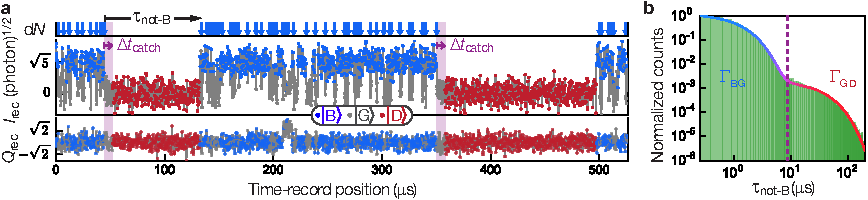
\includegraphics[width=150mm]{intro/2_jumps} \caption[Unconditioned monitoring of quantum jumps in the 3-level system]{\label{fig:jumps} \textbf{Unconditioned monitoring of quantum jumps
in the 3-level system.} \textbf{a,} Typical measurement of integrated,
with duration $T_{\mathrm{int}},$ quadratures $I_{\mathrm{rec}}$
and $Q_{\mathrm{rec}}$ of signal reflected from readout cavity as
a function of time. The color of the dots (see legend) denotes the
state of the atom estimated by a real-time filter implemented with
the FPGAs (see Section\,\ref{subsec:IQ-filter}). On top, the vertical
arrows indicate ``click'' events ($\mathrm{d}N$) corresponding
to the inferred state changing from $\ket{\mathrm{B}}$ to not-$\ket{\mathrm{B}}$.
The symbol $\tau_{\operatorname{not-B}}$ corresponds to the time
spent in not-$\ket{\mathrm{B}}$, which is the time between two clicks
minus the last duration spent in $\ket{\mathrm{B}}$. An advance warning
that a jump to $\ket{\mathrm{D}}$ is occurring is triggered when
\textit{no} click has been observed for a duration $\Delta t_{\mathrm{catch}}$,
which is chosen between 1 and 12$\,\mathrm{\mu s}$ at the start of
the experiment. % 30 consecutive G points before declare D,  30*0.26 = 7.8 us  (2*delta t_mid)
\textbf{b,} Log-log plot of the histogram of $\tau_{\operatorname{not-B}}$
(shaded green) for 3.2 s of continuous data of the type of panel (a).
Solid line is a bi-exponential fit defining jump rates $\Gamma_{\mathrm{BG}}=\left(0.99\pm0.06\,\mathrm{\mu s}\right)^{-1}$
and $\Gamma_{\mathrm{GD}}=\left(30.8\pm0.4\,\mathrm{\mu s}\right)^{-1}$.}
\end{figure*}


\section{Catching the quantum jump\label{sec:Catching-the-quantum}}

Having observed the quantum jumps in the free-running protocol, we
proceed to conditionally actuate the system control tones in order
to tomographically reconstruct the time dynamics of the quantum jump
from $\ket{\mathrm{G}}$ to $\ket{\mathrm{D}}$, see Fig.\,\ref{fig:catch}a.
Like previously, after initiating the atom in $\ket{\mathrm{B}}$,
the FPGA controller continuously subjects the system to the atom drives
($\Omega_{\mathrm{BG}}$ and $\Omega_{\mathrm{DG}}$) and to the readout
tone ($\mathrm{R}$). However, in the event that the controller detects
a single click followed by the complete absence of clicks for a total
time $\Delta t_{\operatorname{catch}}$, the controller suspends all
system drives, thus freezing the system evolution, and performs tomography,
as explained in Section \ref{subsec:Tomography-of-three-level}. Note
that in each realization, the tomography measurement yields a single
+1 or -1 outcome, one bit of information for a single density matrix
component. We also introduce a division of the duration $\Delta t_{\operatorname{catch}}$
into two phases, one lasting $\Delta t_{\mathrm{on}}$ during which
$\Omega_{\mathrm{DG}}$ is left on and one lasting $\Delta t_{\mathrm{off}}=\Delta t_{\operatorname{catch}}-\Delta t_{\mathrm{on}}$
during which $\Omega_{\mathrm{DG}}$ is turned off. As we explain
below, this has the purpose of demonstrating that the evolution of
the jump is not simply due to the Rabi drive between $\ket{\mathrm{G}}$
and $\ket{\mathrm{D}}$.

In Fig.\,\ref{fig:catch}b, we show the dynamics of the jump mapped
out in the full presence of the Rabi drive, $\Omega_{\mathrm{GD}}$,
by setting $\Delta t_{\mathrm{off}}=0$. From $3.4\times10^{6}$ experimental
realizations we reconstruct, as a function of $\Delta t_{\operatorname{catch}}$,
the quantum state, and present the evolution of the jump from $\ket{\mathrm{G}}$
to $\ket{\mathrm{D}}$ as the normalized, conditional GD tomogram
(see Section \ref{subsec:Tomography-of-three-level}). For $\Delta t_{\operatorname{catch}}<2\,\mathrm{\mu s}$,
the atom is predominantly detected in $\ket{\mathrm{G}}$ ($Z_{\mathrm{GD}}=-1$),
whereas for $\Delta t_{\operatorname{catch}}>10\,\mathrm{\mu s}$,
it is predominantly detected in $\ket{\mathrm{D}}$ ($Z_{\mathrm{GD}}=+1$).
Imperfections, due to excitations to higher levels, reduce the maximum
observed value to $Z_{\mathrm{GD}}=+0.9$ (see Section\,\ref{subsec:Error-analysis}). 

\begin{figure}
\centering{}\includegraphics[width=130mm]{intro/3_catch} \caption[Catching the quantum jump mid-flight]{\label{fig:catch}\textbf{Catching the quantum jump mid-flight.}
\textbf{a,} The atom is initially prepared in $\ket{\mathrm{B}}$.
The readout tone ($\mathrm{R}$) and atom Rabi drive $\Omega_{\mathrm{BG}}$
are turned on until the catch condition is fulfilled, consisting of
the detection of a click followed by the absence of click detections
for a total time $\Delta t_{\mathrm{catch}}$. The Rabi drive $\Omega_{\mathrm{DG}}$
starts with $\Omega_{\mathrm{BG}}$, but can be shut off prematurely,
prior to the end of $\Delta t_{\mathrm{catch}}$. A tomography measurement
is performed after $\Delta t_{\mathrm{catch}}$. \textbf{b \& c,}
Conditional tomography revealing the continuous, coherent, and, surprisingly,
deterministic flight (when completed) of the quantum jump from $\ket{\mathrm{G}}$
to $\ket{\mathrm{D}}$. The error bars are smaller than the size of
the dots. The mid-flight time $\Delta t_{\mathrm{mid}}$ is defined
by $Z_{\mathrm{GD}}=0$. The jump proceeds even when $\Omega_{\mathrm{DG}}$
is turned off at the beginning of the flight (panel c), $\Delta t_{\mathrm{on}}=2\,\mathrm{\mu s}$.
Data obtained from $6.8\times10^{6}$ experimental realizations. Solid
lines: theoretical prediction (see Sec.~\ref{subsec:Comparison-between-theory}).
Dashed lines in panel c: theory curves for the $\Delta t_{\mathrm{on}}$
interval, reproduced from panel b. The data suggests that an advance-warning
signal of the jump can be provided by a no-click period for catch
time $\Delta t_{\mathrm{catch}}=\Delta t_{\mathrm{mid}}$, at which
half of the jumps will complete.}
\end{figure}

For intermediate no-click times, between $\Delta t_{\operatorname{catch}}=2\,\mathrm{\mu s}$
and $\Delta t_{\operatorname{catch}}=10\,\mathrm{\mu s}$, the state
of the atom evolves continuously and coherently from $\ket{\mathrm{G}}$
to $\ket{\mathrm{D}}$ --- the flight of the quantum jump. The time
of mid flight, $\Delta t_{\mathrm{mid}}\equiv3.95\,\mathrm{\mu s}$,
is markedly shorter than the Rabi period $2\pi/\Omega_{\mathrm{DG}}=50\,\mathrm{\mu s}$,
and is given by the function $\Delta t_{\text{mid}}=\left(\frac{\Omega_{\mathrm{BG}}^{2}}{2\Gamma}\right)^{-1}\ln\left(\frac{\Omega_{\mathrm{BG}}^{2}}{\Omega_{\mathrm{DG}}\Gamma}+1\right)$,
in which $\Omega_{\mathrm{DG}}$ enters logarithmically (see Section
\ref{sec:thry:3lvl-atom-simple-log}). The maximum coherence of the
superposition, corresponding to $\sqrt{X_{\mathrm{GD}}^{2}+Y_{\mathrm{GD}}^{2}}$,
during the flight is $0.71\pm0.005$, quantitatively understood to
be limited by several small imperfections (see Section\,\ref{subsec:Error-analysis}).

Motivated by the exact quantum trajectory theory, we fit the experimental
data with the analytic form of the jump evolution, $\mathrm{Z}_{\text{GD}}(\Delta t_{\operatorname{catch}})=a+b\tanh(\Delta t_{\operatorname{catch}}/\tau+c)$,
$\mathrm{X}_{\text{GD}}(\Delta t_{\operatorname{catch}})=a'+b'\operatorname{sech}(\Delta t_{\operatorname{catch}}/\tau'+c')$,
and $\mathrm{Y}_{\text{GD}}(\Delta t_{\operatorname{catch}})=0$.
We compare the fitted jump parameters ($a,a',b,b',c,c',\tau,\tau'$)
to those calculated from the theory and numerical simulations using
independently measured system characteristics (see Section \ref{subsec:Comparison-between-theory}).

By repeating the experiment with $\Delta t_{\text{on}}=2\,\mathrm{\mu s}$,
in Fig.~\ref{fig:catch}c, we show that the jump proceeds even if
the GD drive is shut off at the beginning of the no-click period.
The jump remains coherent and only differs from the previous case
in a minor renormalization of the overall amplitude and timescale.
The mid-flight time of the jump, $\Delta t_{\mathrm{mid}}'$, is given
by an updated formula (see Chapter \ref{chap:theoretical-description-jumps}).
The results demonstrate that the role of the Rabi drive $\Omega_{\mathrm{DG}}$
is to initiate the jump and provide a reference for the phase of its
evolution\footnote{A similar phase reference for a non-unitary, yet deterministic, evolution
induced by measurement was previously found in a different context
in: N. Katz, M. Ansmann, R. C. Bialczak, E. Lucero, R. McDermott,
M. Neeley, M. Steffen, E. M. Weig, A. N. Cleland, J. M. Martinis,
and A. N. Korotkov, Science (New York, N.Y.) 312, 1498 (2006).}. Note that the $\Delta t_{\mathrm{catch}}\gg\Delta t_{\mathrm{mid}}$
non-zero steady state value of $X_{\mathrm{GD}}$ in Fig.~\ref{fig:catch}b
is the result of the competition between the Rabi drive $\Omega_{\mathrm{DG}}$
and the effect of the measurement of $\ket{\mathrm{B}}$. This is
confirmed in Fig.~\ref{fig:catch}c, where $\Omega_{\mathrm{DG}}=0$,
and where there is no offset in the steady state value.

The results of Fig.~\ref{fig:catch} demonstrate that despite the
unpredictability of the jumps from $\ket{\mathrm{G}}$ to $\ket{\mathrm{D}}$,
they are preceded by an identical no-click record. While the jump
starts at a random time and can be prematurely interrupted by a click,
the deterministic nature of the flight comes as a surprise given the
quantum fluctuations in the heterodyne record $I_{\mathrm{rec}}$
during the jump --- an island of predictability in a sea of uncertainty. 

\section{Reversing the quantum jump\label{sec:Reversing-the-quantum}}

\begin{figure}
\centering{}\includegraphics[width=130mm]{intro/4_reverse}
\caption[Reversing the quantum jump mid-flight]{\label{fig:reverse}\textbf{Reversing the quantum jump mid-flight.}
\textbf{a,} Bloch sphere of the GD manifold, showing the axis X' for
the jump reversal, defined by the azimuthal angle $\varphi_{\mathrm{I}}$.
The angle of the intervention pulse is $\theta_{\mathrm{I}}$. \textbf{b,}
Success probabilities $P_{\mathrm{G}}$ (purple) and $P_{\mathrm{D}}$
(orange) to reverse to $\ket{\mathrm{G}}$ and complete to $\ket{\mathrm{D}}$
the quantum jump mid-flight at $\Delta t_{\mathrm{catch}}=\Delta t_{\mathrm{mid}}$,
with $\theta_{\mathrm{I}}=\pi/2$, in the presence of the Rabi drive
$\Omega_{\mathrm{DG}}$. The error bars are smaller than the size
of the dots. Black dots: success probability for $\ket{\mathrm{G}}$
(closed dots) and $\ket{\mathrm{D}}$ (open dots) in a control experiment
where intervention is applied at random times along the record, rather
than at $\Delta t_{\mathrm{catch}}$. \textbf{c,} Optimal success
of reverse protocol (purple) as a function of $\Delta t_{\mathrm{catch}}$.
The FPGA controller is programmed with the optimal $\left\{ \theta_{I}\left(\Delta t_{\mathrm{catch}}\right),\varphi_{I}\left(\Delta t_{\mathrm{catch}}\right)\right\} $.
Closed and open dots correspond to $\Delta t_{\mathrm{on}}=\Delta t_{\mathrm{catch}}$
and $\Delta t_{\mathrm{on}}=2\,\mathrm{\mu s}$, respectively. Red
points show the corresponding open-loop (no intervention) results
from Fig.~\ref{fig:catch}b and~c.}
\end{figure}

In Fig.~\ref{fig:reverse}b, we show that by choosing $\Delta t_{\operatorname{catch}}=\Delta t_{\mathrm{mid}}$
for the no-click period to serve as an advance warning signal, we
reverse the quantum jump\footnote{Reversal of quantum jumps have been theoretically considered in different
contexts, see H. Mabuchi and P. Zoller, Phys. Rev. Lett. 76, 3108
(1996) and R. Ruskov, A. Mizel, and A. N. Korotkov, Phys. Rev. B 75,
220501(R) (2007).} in the presence of $\Omega_{\mathrm{DG}}$; the same result is found
when $\Omega_{\mathrm{DG}}$ is off, see Section \ref{subsec:Incoherent-Bright-drive}.
The reverse pulse characteristics are defined in Fig.~\ref{fig:reverse}a.
For $\varphi_{\mathrm{I}}=\pi/2$, our feedback protocol succeeds
in reversing the jump to $\ket{\mathrm{G}}$ with $83.1\%\pm0.3\%$
fidelity, while for $\varphi_{\mathrm{I}}=3\pi/2$, the protocol completes
the jump to $\ket{\mathrm{D}}$, with $82.0\%\pm0.3\%$ fidelity.
In a control experiment, we repeat the protocol by applying the reverse
pulse at random times, rather than those determined by the advance
warning signal. Without the advance warning signal, the measured populations
only reflect those of the ensemble average.

In a final experiment, we programmed the controller with the optimal
reverse pulse parameters $\left\{ \theta_{I}\left(\Delta t_{\mathrm{catch}}\right),\varphi_{I}\left(\Delta t_{\mathrm{catch}}\right)\right\} $,
and as shown in Fig.~\ref{fig:reverse}c, we measured the success
of the reverse protocol as a function of the catch time, $\Delta t_{\mathrm{catch}}$.
The closed/open dots indicate the results for $\Omega_{\mathrm{DG}}$
on/off, while the solid curves are theory fits motivated by the exact
analytic expressions (see Chapter \ref{chap:theoretical-description-jumps}).
The complementary red dots and curves reproduce the open-loop results
of Fig.~\ref{fig:catch} for comparison.

\section{Discussion of main results\label{sec:Discussion-of-main-results}}

From the experimental results of Fig.~\ref{fig:jumps}a one can infer,
consistent with Bohr's initial intuition and the original ion experiments,
that quantum jumps are random and discrete. Yet, the results of Fig.~\ref{fig:catch}
support a contrary view, consistent with that of Schrödinger: the
evolution of the jump is coherent and continuous. Noting the difference
in time scales in the two figures, we interpret the coexistence of
these seemingly opposed point of views as a unification of the discreteness
of countable events like jumps with the continuity of the deterministic
Schrödinger’s equation. Furthermore, although all $6.8\times10^{6}$
recorded jumps (Fig.~\ref{fig:catch}) are entirely independent of
one another and stochastic in their initiation and termination, the
tomographic measurements as a function of $\Delta t_{\mathrm{catch}}$
explicitly show that all jump evolutions follow an essentially identical,
predetermined path in Hilbert space --- not a randomly chosen one
--- and, in this sense, they are deterministic. These results are
further corroborated by the reversal experiments shown in Fig.~\ref{fig:reverse},
which exploit the continuous, coherent, and deterministic nature of
the jump evolution and critically hinge on priori knowledge of the
Hilbert space path. With this knowledge ignored in the control experiment
of Fig.~\ref{fig:reverse}b, failure of the reversal is observed.

In conclusion (see Chapter~\ref{chap:Conclusion-and-perspective}
for an expanded discussion), these experiments revealing the coherence
of the jump, promote the view that a single quantum system under efficient,
continuous observation is characterized by a time-dependent state
vector inferred from the record of previous measurement outcomes,
and whose meaning is that of an objective, generalized degree of freedom.
The knowledge of the system on short timescales is not incompatible
with an unpredictable switching behavior on long time scales. The
excellent agreement between experiment and theory including known
experimental imperfections (see Sec.~\ref{subsec:Comparison-between-theory})
thus provides support to the modern quantum trajectory theory and
its reliability for predicting the performance of real-time intervention
techniques in the control of single quantum systems.

